\documentclass[crop,tikz]{standalone}% 'crop' is the default for v1.0, before it was 'preview'
% \usetikzlibrary{...}% tikz package already loaded by 'tikz' option
\begin{document}

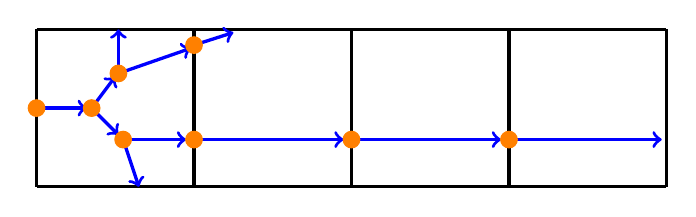
\begin{tikzpicture}[scale=2]
  \draw [step=1.0, very thick] (0,0) grid (4,1);
  
  \draw[->,blue,very thick] (0.05,.5) -- (.32,.5);
  \draw[->,blue,very thick] (0.35,.5) -- (.5,.7);
  \draw[->,blue,very thick] (0.52,.72) -- (.52,1);
  \draw[->,blue,very thick] (0.52,.72) -- (.98,.88);
  \draw[->,blue,very thick] (1,.9) -- (1.25,.98);
  \draw[->,blue,very thick] (0.35,.5) -- (.52,.33);
  \draw[->,blue,very thick] (0.55,.3) -- (.95,.3);
  \draw[->,blue,very thick] (0.55,.3) -- (.65,0);
  \draw[->,blue,very thick] (1.05,.3) --(1.95,.3);
  \draw[->,blue,very thick] (2.05,.3) -- (2.95,.3);
  \draw[->,blue,very thick] (3.05,.3) -- (3.97,.3);
  %\draw[->,blue,very thick] (3.55,.3) -- (3.97,0.3);
  
  \filldraw[orange] (0,.5) circle (1.5pt);
  \filldraw[orange] (0.52,.72) circle (1.5pt);
  \filldraw[orange] (1.,.9) circle (1.5pt);
  \filldraw[orange] (0.35,.5) circle (1.5pt);
  \filldraw[orange] (0.55,.3) circle (1.5pt);
  \filldraw[orange] (1,.3) circle (1.5pt);
  \filldraw[orange] (2,.3) circle (1.5pt);
  \filldraw[orange] (3,.3) circle (1.5pt);
  %\filldraw[orange] (3.5,.3) circle (1.5pt);

\end{tikzpicture}
\end{document}